% !TeX spellcheck = en_GB
%!TEX TS-program = xelatex
%!BIB TS-program = biber
\chapter{Clustering Analysis of Partitions}\label{chap:p4}

\section*{Statement of Contribution}
	This chapter includes a co-authored journal. The bibliographic details of the published chapter are:
\begin{itemize}
	\item Javanbakht, Z, Hall, W \& Öchsner, A (2017), “The Effect of Partitioning on the Clustering Index of Randomly-Oriented Fiber Composites: A Parametric Study”, Defect and Diffusion Forum 380, pp. 232–241.
\end{itemize}
	My contribution as the corresponding author to the paper involved: undertaking literature review, classifying the necessary theoretical backgrounds and models, developing the programming code, analysing and discussing the finite element results, drawing figures, preparing tables, writing and editing the manuscript according to my supervisors’ comments.

\Zia\\
\Wayne\\
\vfill
\newpage

% --------------------------------------------------------------------------------------------------

\paragraph{Title} The Effect of Partitioning on the Clustering Index of Randomly-Oriented fibre Composites: A Parametric Study

\paragraph{Abstract} In the current study, five cases of fibre distributions are considered in a fibre-reinforced composite: one random, three partitioned (one uniform and two biased cases), and one aligned case for benchmarking. The finite element method and the principal component analysis were used to interpret the results of orientation tensors and detect any possible clusterings of a representative volume element (RVE). The obtained effective conductivity values were extensively controlled by the fibre volume fraction. At the same time, the uniformity of the random distributions could be recognized. Cross-partition resistance was also detected for the partitioned cases which contributed to a reduced heat transfer capability. Finally, the clustering indexes did not show a direct correlation with the conductivity results, and thus a case-by-case investigation is recommended to consider the anisotropic aspects of a microstructure.

\paragraph{Keywords} Finite element method; Reinforced composites; Thermal analysis; fibre clustering.

\section{Introduction}
	A combination of two or more materials---distinct in properties and boundaries---is referred to as a composite material. Often, the compliant material with the greatest volume is the matrix while other stiffer and stronger constituents are generally called inclusions\,\footnote{There are exceptions to this statement, e.g., the volume fraction of fibres in aerospace-grade composites are unusually higher than that of the matrix.}. The properties of the final material depend on the properties of all its constituents; geometry, distribution, orientation, and concentration of the reinforcements; and the quality of the matrix-inclusion interface~\autocite{Altenbach.2010}. Inclusions are used in the form of fibres, laminates, particles, or a combination of them to produce various classes of composites~\autocite{Jones.1999} among which randomly-oriented fibres are of interest in the current study.

	Various analytical, numerical and statistical approaches are proposed in the literature to foresee the properties of a composite. In most of such procedures a randomly-oriented---yet uniform---distribution of fibres is assumed, see for instance~\autocite{Lu.2014,Javanbakht.2016b,Javanbakht.2016}. However, under some practical manufacturing conditions, e.g., poor mixing in injection moulding, or high volume fraction of fibres, uniformity of dispersion is lost~\autocite{Kataoka.2000}. Namely, fibre-fibre interactions within the composite may affect the dispersion state, and create non-uniform concentration regions of fibres. In such a domain with non-homogeneous fibre distribution, fibres in the high concentrations regions co-orient themselves, and thus a preferred orientation is formed---called fibre clustering, albeit particle clustering is also possible~\autocite{Jack.2005,Tszeng.1998,Tewari.2004}.
	
	In terms of direction, an orientation cluster is formed by the fibres of a region which share the same orientation state~\autocite{Folgar.1984}. Kanatani~\autocite{Kanatani.1984} introduced three frame indifferent forms for capturing the statistical directional data and tested their application on inter-particular contact distribution of a 2D granular material. Tensorial representation of fibre orientation was introduced in \autocite{Advani.1987,Advani.1990} to ultimately quantify fibre clustering.
	
	Orientation tensors were measured and calculated for injection-moulded tensile samples which indicated a flow-direction alignment close to the mould wall while a more random dispersion exists in the middle of the specimens~\autocite{Lee.2003}. Such measurements are crucial for characterizing the physical properties of the specimen based on its internal structure. For instance, elastic properties of short-fibres can be extracted more accurately from homogenization of the micro-computer tomography images by observing fibre orientations~\autocite{Muller.2015}. Additionally, similarities of fibre alignment phenomenon between micro- and nano-scales promise an exchangeable knowledge basis which further emphasise on the importance of the topic~\autocite{Fan.2005,Yang.2010}.
	
	Herein, the mixing-analogy method is used to indicate the orientation clustering, first introduced in~\autocite{Ranganathan.1990}, by numerically examining the incorporated tensorial representation. Four cases of moderate fibre volume fractions for randomly-oriented composites were considered by means of a planar prototype as well as an aligned model for benchmarking. A high contrast property is assumed for the composite constituents to take into account the sensitivity of such mediums to fibre clustering~\autocite{Kataoka.2000}. A list of used symbols is also provided in Table~\ref{table:symbols}.
\begin{table}[!h]
\centering
\caption{List of symbols}\label{table:symbols}
\begin{tabular}{>{\centering}p{0.15\textwidth}>{\small}p{0.7\textwidth}}
\toprule\noalign{\smallskip}
$\alpha$           & thermal conductivity contrast\\
$\beta$           & fibre aspect ratio\\
$\gamma$           & mesh density\\
$\vartheta^\prime$   & rotation of the principal direction transformation\\
$\zeta_{\text{f}}$  & volume fraction of the fibre\\
$\lambda_i$        & $i$-th eigenvalue\\
$\psi$             & probability distribution function\\
$\Delta T$       & prescribed temperature gradient\\
$\Delta z$         & length over which temperature gradient is formed, i.e., the distance between the boundary edges\\
$a$                & element edge length\\
$k_{\text{eff}}$   & effective thermal conductivity of the composite\\
$k_{\text{f}}$     & thermal conductivity of the fibre\\
$k_{\text{m}}$     & thermal conductivity of the matrix\\
$A_0$              & cross-sectional area perpendicular to direction of the flux\\
$\dot{Q}$          & total heat flux magnitude\\
$\tena{e}_i$       & orthonormal unit basis\\
$\tena{e}_i^\prime$     & orthonormal unit basis in the principal direction\\
$\tena{d}$         & fibre direction vector\\
$\tenb{H}$         & orientation second-order tensor\\
$\tenb{H}^\prime $      & orientation second-order tensor in the spectral form\\
$\tenb{Q}$         & transformation second-order tensor\\
\noalign{\smallskip}\bottomrule\noalign{\smallskip}
\end{tabular}
\end{table}

\section{Tensorial Representation of Planar Orientation State}
\begin{figure}[!h]
%\tdplotsetmaincoords{60}{110}
\centering
%\begin{tikzpicture}[scale=4,tdplot_main_coords]
%%define polar coordinates for some vector
%\pgfmathsetmacro{\rvec}{1.2}
%\pgfmathsetmacro{\varthetavec}{40}
%\pgfmathsetmacro{\varphivec}{50}
%
%\coordinate (O) at (0,0,0);
%
%%determine a coordinate (P) using (r,\vartheta,\varphi) coordinates.  This command
%%also determines (Pxy), (Pxz), and (Pyz): the xy-, xz-, and yz-projections
%%of the point (P).
%%syntax: \tdplotsetcoord{Coordinate name without parentheses}{r}{\vartheta}{\varphi}
%\tdplotsetcoord{P}{\rvec}{\varthetavec}{\varphivec}
%\tdplotsetcoord{Punit}{\rvec/3}{\varthetavec}{\varphivec}
%
%%draw figure contents
%%--------------------
%
%%draw the main coordinate system axes
%\draw[thick,->] (0,0,0) -- (1,0,0) node[anchor=north east]{$1$};
%\draw[thick,->] (0,0,0) -- (0,1,0) node[anchor=west]{$2$};
%\draw[thick,->] (0,0,0) -- (0,0,1) node[anchor=south]{$3$};
%
%%draw a vector from origin to point (P) 
%\draw[color=black!50,line width=0.2cm] (O) -- (P) node [color=black,above=-0.1cm] {fibre};
%\draw[color=black,dash dot] (O) -- (P);
%\draw[-stealth,very thick, label=fibre] (O) -- (Punit) node [below right] {$\tena{d}$};
%
%%draw projection on xy plane, and a connecting line
%\draw[dashed] (O) -- (Pxy);
%\draw[dashed] (P) -- (Pxy);
%
%%draw the angle \varphi, and label it
%%syntax: \tdplotdrawarc[coordinate frame, draw options]{center point}{r}{angle}{label options}{label}
%\tdplotdrawarc{(O)}{0.2}{0}{\varphivec}{anchor=north}{$\varphi$}
%
%
%%set the rotated coordinate system so the x'-y' plane lies within the
%%"theta plane" of the main coordinate system
%%syntax: \tdplotsetthetaplanecoords{\varphi}
%\tdplotsetthetaplanecoords{\varphivec}
%
%%draw theta arc and label, using rotated coordinate system
%\tdplotdrawarc[tdplot_rotated_coords]{(0,0,0)}{0.5}{0}{\varthetavec}{anchor=south west}{$\vartheta$}
%
%%draw some dashed arcs, demonstrating direct arc drawing
%%\draw[dashed,tdplot_rotated_coords] (\rvec,0,0) arc (0:90:\rvec);
%%\draw[dashed] (\rvec,0,0) arc (0:90:\rvec);
%\end{tikzpicture}
  	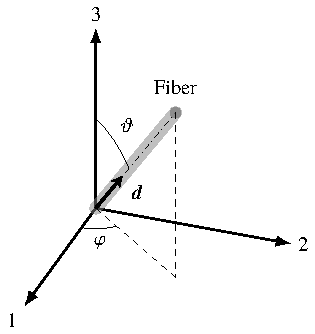
\includegraphics[scale=1]{direction_vector}
\caption{Representation of the orientation of a general fibre in the 3D space using a unit vector~$\tena{d}$}\label{fig:vector}
\end{figure}%
	The orientation of each fibre is denoted by a unit vector ($\tena{d}=\tena{d}(\vartheta,\varphi)$) as a 3D spatial function, see Fig.~\ref{fig:vector}, which can be readily specified using the summation convention:
	\begin{equation}
	\tena{d}=d_i\tena{e}_i,\qquad i=1,2,3,
	\end{equation}
	where $\tena{e_i}$ is the $i$-th basis unit vector of the coordinate system, and  $d_i$ is the $i$-th component of the unit vector $\tena{d}$. This presentation reduces to summation over two indexes ($i=1,2$) for a planar coordinate system, i.e., $\tena{d}=\tena{d}(\varphi)$.

	The statistical distribution of fibres in the vicinity of a unit vector is specified by the probability distribution function ($\psi=\psi(\tena{d})$):
	\begin{equation}
	\psi(\vartheta,\varphi)=\delta(\vartheta-\frac{\uppi}{2})\psi_\varphi(\varphi),
	\end{equation}
	where $\delta$ is the Dirac delta function and $\psi$ is the planar probability distribution function. Consequently, the 2nd-order planar orientation tensor ($\tenb{H}$) can be defined as~\autocite{Advani.1987}:
\begin{equation}\label{eq:one}
H_{ij}=\int_{0}^{2\uppi}\psi(\varphi)d_id_j \dif\varphi,
\end{equation}
where $d_i$ and $d_j$ are the $i$-th and $j$-th components of the unit vector $\tena{d}$, respectively. A discretised formulation of Eq.~\eqref{eq:one} directly reveals the components of the planar orientation tensor for a specific region containing $N_\text{f}$ number of fibres~\autocite{Ranganathan.1990}:
\begin{equation}
H_{ij}\approx\frac{1}{N_\text{f}}\sum_{k=1}^{N_\text{f}}p_i^kp_j^k,
\end{equation}
where it basically provides the average orientation tensor component of the entire sample ($\overline{\overline{H_{ij}}}$) if the total number of fibres in the sample is used. Note that since the orientation tensor is symmetric:
\begin{equation}
H_{ij}=H_{ji},
\end{equation}
and to fulfil the normalization condition of $\psi_\varphi$:
\begin{equation}
H_{ii}=1,
\end{equation}
thus there are only two independent components in the planar orientation tensor, e.g., $H_{11}$, and $H_{12}$. Namely, $H_{11}$ quantifies the proportion of alignment along the 1-axis and $H_{12}$ indicates the deviation of the coordinate axes from the principal directions of the orientation tensor.


Since the second ordered orientation tensor is symmetric, there exists an orthonormal basis ($\tena{e}_i^\prime$) along which the spectral form ($\tenb{H}^\prime$) of the orientation tensor ($\tenb{H}$) can be acquired~\autocite{Bertram.2015}:
\begin{equation}
\tenb{H}^\prime=\lambda_i\tena{e}_i^\prime\otimes\tena{e}_i^\prime,
\end{equation}
where $\lambda_i$ are the real eigenvalues and $\tena{e}_i^\prime$ are the normed eigenvectors forming the basis of the orthonormal coordinate system. A unique rotation $\tenb{Q}$ is used to transform the orientation tensor, by an angle equal to $\vartheta^\prime$, to the principal directions to obtain:
\begin{equation}
\mat{H}^\prime=\left[\begin{matrix}
\lambda_1& 0 \\
0 & \lambda_2\\
\end{matrix}
 \right].
\end{equation}
An ellipse can be used to illustrate the principal components. The axes of the ellipse are the principal directions and their length are proportional to the degree of the orientation along the their directions. Finally, the major axis denotes the preferred direction of the fibres. Such an ellipse can be used to graphically represent the orientation of fibres in a selected region. Note that for highly aligned fibres, the minor axis of the ellipse is diminished and only a line along the major axis will remain. In contrast, a circle indicates that no preferred directions exist~\autocite{Advani.1990,Advani.1987}.\\

\section{Clustering Index}
A sample of total $N_\text{f}$ short fibres is subdivided into $N_\text{p}$ partitions:
\begin{equation}
N_\text{f}=\sum_{l=1}^{N_\text{p}}N_{\text{f}\,l},
\end{equation}
where $N_{\text{f}\,l}$ is the total number of fibres in the $l$-th partition. The orientation state of the $l$-th partition ($\overline{H_{ij}^l}$) is:
\begin{equation}
\overline{H_{ij}^l}=\frac{1}{N_{\text{f}\,l}}\sum_{k=1}^{N_{\text{f}\,l}}H_{ij}^{kl}.
\end{equation}
and the orientation state of the whole sample is:
\begin{equation}
\overline{\overline{H_{ij}}}=\frac{1}{N_\text{f}}\sum_{k=1}^{N_\text{f}}H_{ij}^k.
\end{equation}
From the mixing-analogy method, the clustering index $\text{[CI]}$ is defined as~\autocite{Ranganathan.1990}:
\begin{equation}
{\text{[CI]}}_{ij}=\frac{N_\text{p}-1}{N_\text{f}-1}\;\frac{[\upsigma_\text{bp}^2]_{ij}}{[\upsigma_\text{t}^2]_{ij}},
\end{equation}
where $[\upsigma_\text{bp}^2]_{ij}$ is the variance between the partitions, and $[\upsigma_\text{t}^2]_{ij}$ is the total variance. Finally, the type-1 clustering index can be expressed in terms of the orientation state as follows:
\begin{equation}
{\text{[CI]}}_{ij}=1-\dfrac{
\sum\limits_{l=1}^{N_\text{p}}\sum\limits_{k=1}^{N_{\text{f}\,l}}(H_{ij}^{kl}-\overline{H_{ij}^l})^2
}{
\sum\limits_{l=1}^{N_\text{p}}\sum\limits_{k=1}^{N_{\text{f}\,l}}(H_{ij}^{kl}-\overline{\overline{H_{ij}^l}})^2
},
\end{equation}
where the numerator indicates the sum of the variances within each partition and the denominator is the variance of the whole RVE.
\red
\section{Micro-mechanical Model for Discontinuous Fibres}
	The extension of the Eshelby model~\autocite{Eshelby.1957,Eshelby.1961} to heat transfer problems is the Hatta-Taya model~\autocite{Hatta.1985,Taya.1989}. In either model, the equivalent inclusion technique is adopted by introducing a transformation tensor that creates a homogeneous medium from the composite with heterogeneities. Thereof, an eigen-quantity~\autocite{Mura.1987} is related to its constraint counterpart. Such an approach is common in Duhamel-Neumann type equations~\autocite{Javanbakht.2019b,Ghosh.2011}. In its classic derivation, such a relation is established by the Eshelby tensor, which depends on the geometry of the inclusions. Herein, ellipsoidal inclusions (Eshelby's template for inclusions) were adjusted to properly represent short fibres. The three semi-diameters $a_1$, $a_2$, and $a_3$ of spheroids are named along the axis of the coordinate system $\left\{\tena{e}_i\right\}\equiv\left\{\tena{e}_i\right\}_{i=1}^3$. Short fibres are considered as oblate spheroids ($a_1=a_2\ll a_3$) in this model, and the components of the Eshelby tensor are explicitly calculated as \begin{subequations}
		\begin{alignat}{2}
			S_{11}=S_{22}&=\frac{\beta}{2\sqrt{(\beta^2-1)^3}}\left(\beta\sqrt{\beta^2-1}-\cosh^\inv\beta \right),\\
			S_{33}&=1-2S_{22},
		\end{alignat}
		\end{subequations}
	where $\beta\equidef\sfrac{a_3}{a_2}$ is the aspect ratio of the fibres.

	In the formulation of Hatta-Taya model for 2D (on the 1-3 plane), the angle $\alpha$ denotes the range of fibre distribution and $\theta$ is the angle of the fibres, i.e., $0\le \alpha\le\sfrac{\pi}{2}$ and $-\alpha\le \alpha\le\alpha$. The $\rho\equiv\rho(\theta)$ function defines the number of fibres per unit area of the $\mathbb{S}^2$ unit sphere in 3D, which reduces to $\mathbb{S}^1$ unit circle for 2D. In order to model the aligned fibre case, $\alpha\rightarrow 0$ and $\rho\equimust\delta(\theta)$ in which $\delta(\theta)$ is the Kronecker delta generalised function. Furthermore, assuming isotropic materials for both fibre ($\tenb{k}_\text{f}\equiv k_\text{f}\unitb$) and matrix ($\tenb{k}_\text{m}\equiv k_\text{m}\unitb$) phases, the auxiliary tensor
	\begin{equation}
		\tenb{A}\equidef (k_\text{f}-k_\text{m})\unitb\scp\tenb{S}+k_\text{m}\unitb,
	\end{equation}
	is used along with the Eshelby tensor to calculate
	\begin{subequations}
	\begin{alignat}{3}
		Q_1^*        &\equidef (k_\text{m}-k_\text{f})A_{11}^\inv,\\
		Q_3^*        &\equidef (k_\text{m}-k_\text{f})A_{33}^\inv,\\
		Q_1^\text{C} &\equidef (k_\text{m}-k_\text{f})S_{11}A_{11}^\inv,\\
		Q_3^\text{C} &\equidef (k_\text{m}-k_\text{f})S_{33}A_{11}^\inv.
	\end{alignat}
	\end{subequations}
	Finally, the axial (along the 3-axis) and transverse (along the 1-axis) effective properties are calculated by
	\begin{subequations}
	\begin{alignat}{2}
		k_\text{axial} &= k_\text{m}\left( 1 - \frac{\zeta_{\text{f}}Q_3^*}{\zeta_{\text{f}}Q_3^\text{C}}   \right),\\
		k_\text{trans} &= k_\text{m}\left( 1 - \frac{\zeta_{\text{f}}Q_1^*}{1+\zeta_{\text{f}}Q_1^\text{C}}   \right).
	\end{alignat}
	\end{subequations}
	


\bl
\section{Methodology}
In the current study, the numerical solutions were obtained by means of the finite element method~\autocite{Ochsner.2013,Oechsner.2016,Javanbakht.2017c}. The MSC.Marc (version 2017.0) commercial package along with its Python scripting capability was used to automate the mesh generation, job submission, and post-processing stages of the study. Moreover, object oriented programming is used to encapsulate the code for the RVE and fibre class of objects~\autocite{Javanbakht.2017}.
\begin{figure}[!h]
\centering
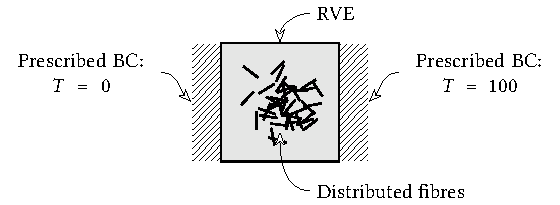
\includegraphics[scale=1]{ddf3_RVE.pdf}
\caption{Schematic illustration of the RVE prototype}\label{fig:RVE}
\end{figure}%

A planar thermal analysis was carried out for each case using a uniform mesh for the matrix consisting of type 39 four-node, isoparametric, arbitrary quadrilateral finite elements with embedded straight 2-node link/truss element as fibres.


The periodicity condition was established for the $20\times20$ planar RVE in which embedded short fibres (with a length equal to $5$) were distributed, see Fig.~\ref{fig:RVE}. Note that dimensionless values were used throughout the investigation. An aspect ratio of $40$ was acquired for the fibres, i.e., a fibre length of $5$ and a diameter of $0.125$, to stay within the range of $20$\thinspace--\thinspace$60$ aspect ratios of the short fibres~\autocite{Kalpakjian.2010}. Although the analysis was carried out in the 2D space, it was assumed that the RVE has a uniform thickness equal to the diameter of the fibres. A high material contrast of $600$ was assumed for the fibre to matrix thermal conductivity ratio; unit thermal conductivity was assigned to the matrix.\red\ As the length of the fibres is a set value, the number of required fibres can be readily calculated for a specific fibre volume fraction. Note that the matrix volume is used for this calculation, i.e., the nominal fibre volume fraction is used instead of the true fibre volume fraction, see~\autocite{Javanbakht.2016b}.\bl

The boundary conditions can highly affect the results of a finite element analysis~\autocite{Javanbakht.2017b}. More specifically, the best results for computational analysis of a periodic fibre-reinforced composite, undergoing heat conduction, is acquired using prescribed temperature boundary conditions~\autocite{Islam.1999}. Therefore, a temperature difference of 100 is applied to the right-hand boundary nodes which results in a reaction heat flux on the same edge, see Fig.~\ref{fig:RVE}. Fourier's law is used to calculate the effective thermal conductivity of the RVE~\autocite{Fiedler.2009}:
\begin{equation}
k_{\text{eff}}=\frac{\dot{Q}}{A_0}\cdot\frac{\Delta z}{\Delta T},
\end{equation}%
where $k_{\text{eff}}$ is the effective thermal conductivity of the RVE, $\dot{Q}$ is the sum of the generated reaction fluxes on the right-hand boundary, $A_0$ is the assumed cross-sectional area perpendicular to direction of the flux, $\Delta z$ is the distance between the edges of the sample, and $\Delta T$ is the prescribed temperature gradient.  

\paragraph{Case studies} The prototype RVE was used to distribute the fibres based on five possible cases (Fig.~\ref{fig:case}):
\begin{enumerate}[itemsep=0cm]
\item uniform randomly-oriented without partitioning,
\item uniform randomly-oriented with partitions,
\item non-uniform randomly-oriented with partitions (downward bias), 
\item non-uniform randomly-oriented with partitions (leftward bias), and
\item  $30^\circ$ aligned fibres with respect to the horizontal axis.
\end{enumerate}
\begin{figure}[!h]
\centering
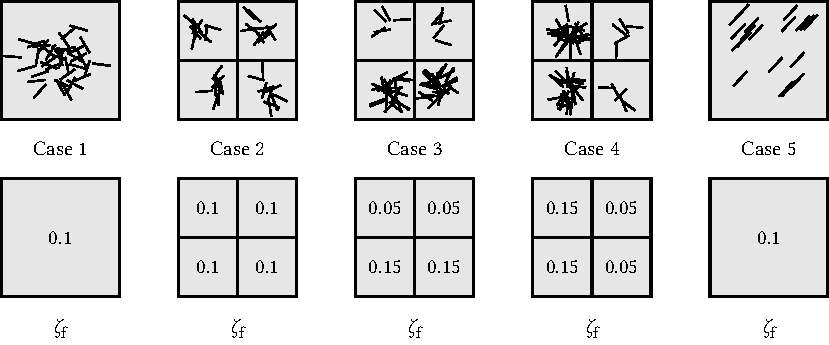
\includegraphics[scale=1]{case}
\caption{Five cases of randomly-oriented fibre distributions and one aligned case schematically illustrated with their corresponding fibre volume fractions}\label{fig:case}
\end{figure}%
The partitioning was done by dividing each edge by half resulting in four partitions in total, i.e., four $5\times5$ partitions. The average fibre volume fraction is the same in each case and the periodicity condition is applied to all the edges, i.e., no penetration across the inner edges in the partitioned cases is allowed. The simulations were repeated ten times for each case while the incorporated algorithm updated the fibre distribution in each job re-submission. The algorithm chooses two random coordinates for nodes, corrects the length of the fibre element, and ensures that the periodicity condition is fulfilled. This is done by cutting and transferring the excess parts of fibre elements to the appropriate edges. Note that fibre overlap is allowed during the mentioned process.




\red 
	\paragraph{Model validation} The results in~\autocite{Fu.2003,Choy.1994} were provided for injection moulded samples made of poly(ether ether ketone) (PEEK) matrix and carbon fibres. Although the through-thickness variation of fibre orientation existed, it was shown that the Hatta-Taya model~\autocite{Hatta.1986,Taya.1989} and the lamination analogy model~\autocite{Clyne.2019} both provide a good agreement with the results. Herein, the Hatta-Taya model was used to benchmark the computational model. To this end, the material properties of~\autocite{Fu.2003,Choy.1994} where used, i.e., the component contrast of $\alpha\equiv\sfrac{k_\text{f}}{k_\text{m}}=32$ ($k_\text{f}=8\,\sfrac{k_\text{trans}}{k_\text{m}}$), and the aspect ratio of $\beta\equiv\sfrac{L}{D}=17$ ($D=6\,\mupmu m$)~\autocite{Choy.1992} were used for aligned short fibres along the heat flux. The dimensions of the RVE were $1\times 1\times0.01\,\text{mm}^3$, which makes the computations effortless.
	
	The response of the FE prototype for aligned short fibres along with the values of the Hatta-Taya model are depicted in Fig.~\ref{fig:ddf3_val}. It can be seen that the current model shows a good correlation with the Hatta-Taya model for a wide range of fibre volume fractions. At higher fractions of fibres, the computational model underestimates the effective thermal conductivity.
\begin{figure}[!h]{}
  \centering
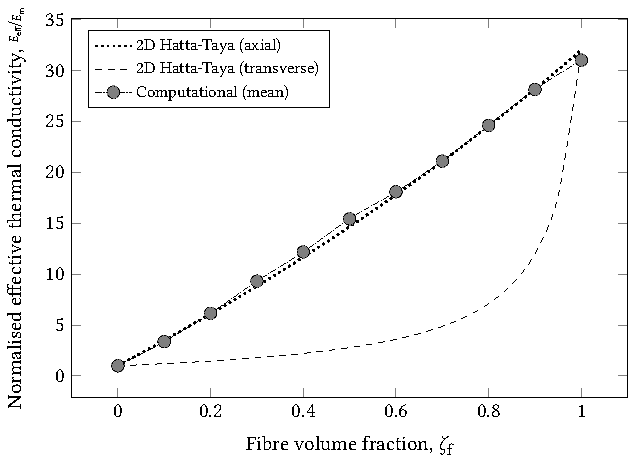
\includegraphics[scale=0.9]{ddf3_validation}
  \caption{Validation of the model with the results provided in~\autocite{Fu.2003,Choy.1994}}
  \label{fig:ddf3_val}
\end{figure}	
	
 	In Table~\ref{table:ddf3_validation}, the percentage relative error of the computational model with respect to the axial thermal conductivity of the Hatta-Taya model is presented. The computational results show a very good agreement with the benchmark analytical model. The percentage relative error remains below 6\%. 
 	%This behaviour can be attributed to the saturation of the 2D model. Namely, since the model is planar and fibre overlap is allowed, a direct contact between the fibres is quickly established---even at low fibre volume fractions. Therefore, a quick rise in thermal conductivity is observed. Nevertheless, this effect tends to be milder as the volume fraction increases because a thermal conductivity path is already established. 

\begin{table}[!h]
\centering
\caption{Effective thermal conductivity results of the computational model against results of the Hatta-Taya micromechanical model.}\label{table:ddf3_validation}
\small
\begin{tabular}{*{4}{P{0.07\textwidth}}P{0.1\textwidth}}
\toprule
  $\zeta_{\text{f}}$ \bfs{(\%)}
& {$\frac{k_\text{trans}}{k_\text{m}}$} 
& {$\frac{k_\text{axial}}{k_\text{m}}$} 
& {$\frac{k_\text{comp}}{k_\text{m}}$} 
& $e_\text{comp}$ \bfs{(\%)}
\\
\toprule
%10 &1.2091  &3.4895 & 3.3645 &  3.58\\
%20 &1.4665  &6.0903 & 6.1566 & -1.09\\
%30 &1.7912  &8.8102 & 9.3042 & -5.61\\
%40 &2.2135  &11.6575& 12.1725& -4.42\\
%50 &2.7853  &14.6414& 15.4221& -5.33\\
%60 &3.6030  &17.7719& 18.0701& -1.68\\
%70 &4.8687  &21.0601& 21.0883& -0.13\\
%80 &7.0893  &24.5183& 24.6012& -0.34\\
%90 &12.0000 &28.1599& 28.1179&  0.15\\
%100&32.0000 &32.0000& 30.9953&  3.14\\
10 &1.21  &3.49 & 3.36 &  3.58\\
20 &1.47  &6.09 & 6.16 & -1.09\\
30 &1.79  &8.81 & 9.30 & -5.61\\
40 &2.21  &11.66& 12.17& -4.42\\
50 &2.78  &14.64& 15.42& -5.33\\
60 &3.60  &17.77& 18.07& -1.68\\
70 &4.87  &21.06& 21.09& -0.13\\
80 &7.09  &24.52& 24.60& -0.34\\
90 &12.00 &28.16& 28.12&  0.15\\
100&32.00 &32.00& 30.99&  3.14\\
 \bottomrule
\end{tabular}
\end{table}	

	The reported experimental value~~\autocite{Choy.1994} on the other hand is lower than both Hatta-Taya and the computational model. The normalised thermal conductivity was 4.5 (measured on the surface) along the longitudinal axis of the coupon for a fibre content of $\zeta_{\text{f}}=0.24$. The fibres were oriented with a 15--20\textsuperscript{$\circ$} angle with respect to the longitudinal axis. The relative axial conductivity improved to $7.2560$ while there was no contribution towards transverse conductivity; this is in accordance with the previously reported results in~\autocite{Javanbakht.2016b}. By transforming the computational results of Table~\ref{table:ddf3_validation} using an average angle of 17.5\textsuperscript{$\circ$}, the normalised thermal conductivity of 6.6903 was obtained, which has about 48.67\% error relative to the experimental value. The manufacturing method was injection moulding, which causes higher alignment on the surface than the mid layer. However in the computational model, the exact length and orientation distribution of the fibres were ignored and only the expected (average) values were used. Similarly, the Hatta-Taya model considers neither the misalignment of fibres nor various fibre aspect ratios. For better results, the exact distributions should be considered in the computational model, see Chapter~\ref{chap:p6}. Nevertheless, having in mind the shortcomings of the current prototype, a \textit{comparative} study could be easily conducted; the cases illustrated in Fig.~\ref{fig:case} was selected for comparison and the results are presented in the following section.
	

	


	
	
	
	
	
	
	
	
	
	
	
	
	
%	In order to capture the orientation of the fibres, the cumulative orientation distribution function~\autocite{Choy.1994}
%	\begin{alignat}{3}
%		F(\theta)&\equidef \frac{1-\exp{(-\lambda\theta)}}{1-\exp{(-\lambda\sfrac{\pi}{2})}},& \qquad\qquad\text{with} &\quad 0\le\theta\le\frac{\pi}{2},
%	\end{alignat}
%	is used whose expected (mean) value is
%	\begin{equation}
%	    \overline{\theta}=\frac{1}{\lambda}-\frac{\pi }{2\,\left(\exp{(\frac{\pi \,\lambda}{2})}-1\right)},
%	\end{equation}
%	where $\lambda$ is the parameter that defines the distribution and varies from 0 to $\infty$ for randomly oriented and fully aligned fibres, respectively.
	


\bl

	\paragraph{Sensitivity analysis} Following the same approach used for model validation, the prototype is updated to a high contrast material $\alpha=600$ and an aspect ratio of $\beta=40$. The benchmark value was the Hatta-Taya model for aligned short fibres along the heat flux. Moreover, mesh sensitivity analysis was carried out for a range of mesh densities, from 1 to 35, where the uniform mesh density~$\gamma$ was defined for a mesh consisting of $\ell_\text{mesh}$ by $\ell_\text{mesh}$ square matrix elements~\autocite{Javanbakht.2018}:
	\begin{equation}
	\gamma\equidef\frac{1}{\ell_\text{mesh}}.
	\end{equation}
	With an an RVE of $10\times 10\times 1$, the sensitivity analysis did not reveal any anomalies. Moreover, the normalised effective conductivity was obtained with percentage relative error of -7.32\% with respect to the benchmark value of 28.98. This underestimation was obtained from a mesh density of 20 and produced an approximation error~\autocite{Chapra.2015} of around 0.12\%, see Fig.~\ref{fig:sensitivty}. For the other cases of the current study, the same RVE and mesh refinement were used for which the results are provided in the following section.
	
\begin{figure}[h]{}
  \centering
%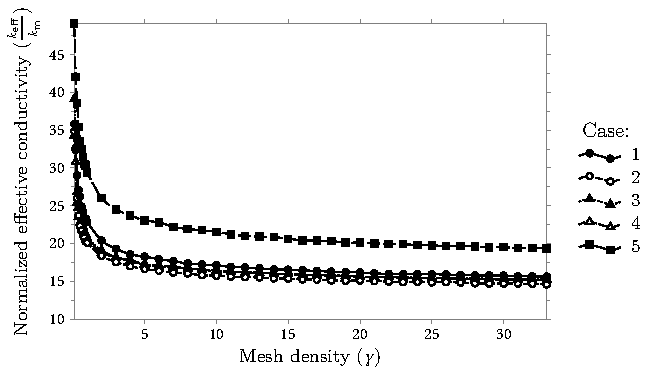
\includegraphics[scale=1]{sens}
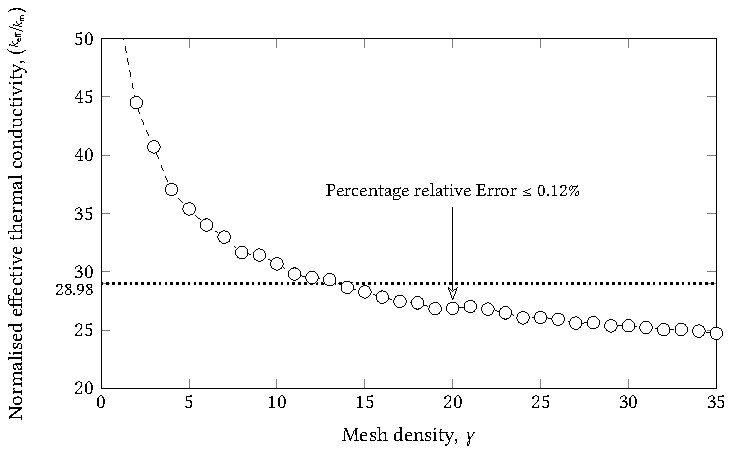
\includegraphics[scale=1]{ddf3_mesh_sens}
  \caption{Sensitivity analysis of normalised effective thermal conductivity versus mesh density in the high contrast FE prototype with aligned fibres}
  \label{fig:sensitivty}
\end{figure}



\red
\section{Results and Discussion}
	The clustering indices ${\text{[CI]}}_{11}$ and ${\text{[CI]}}_{12}$ correspond to the $H_{11}$ and $H_{12}$ components of the orientation tensor, respectively. In any coordinate systems (other than the principal one), the $H_{12}$ component denotes the deviation of the fibre orientations from the 1-axis. Therefore, its corresponding clustering index increases by increasing the difference in the angle of the fibres from one partition to another. On the other hand, $H_{11}$ denotes the strength of the orientation; a stronger orientation has more fibres along 1-axis, and thus $H_{11}$ increases. The respective clustering index ${\text{[CI]}}_{11}$ increases by increasing the difference in the strength of the orientations between partitions. In summary, by the aforementioned indices, clustering of fibres could be quantified in terms of discrepancy in strength and orientation. Note that higher values of clustering indicate more randomness while negligible values represent a more uniform distribution, see~\autocite{Ranganathan.1990} for some examples in this regard. 
	
	It is worth mentioning that since a statistical approach is adopted in the calculation of clustering indices, increasing the number of fibres in each partition would improve the results. From another point of view, one could change the number of partitions\,\footnote{In terms of number of partitions obviously the minimum number is two.} in order to include an adequate number of fibres. This particular number varies case by case, and thus a sensitivity analysis could reveal the exact minimum number.  Otherwise, having a number of fibres around 2--3 order of magnitude seems adequate for typical clustering analyses~\autocite{Ranganathan.1990}.
	
	Herein, an attempt was made to see if clustering indices could be meaningfully related to the effective thermal properties of discontinuous fibre-reinforced composites. To this end, five cases were considered. The temperature gradient was applied to each case, and the reaction heat flux was used to calculate the dimensionless normalised effective conductivity ($\sfrac{k_{\text{eff}}}{k_{\text{m}}}$), see Table~\ref{table:summary}. Case 5 was the $30^\circ$ aligned fibres with respect to the horizontal axis, which showed the highest effective conductivity. The values of other cases vary between 8.42 and 11.36, which can be attributed to the random nature of their fibre generation. Nevertheless, case 4 results in the lowest conductivity value, which is due to the fact that its rightmost partitions act as a barrier against the conduction because of their low fibre volume fractions.\bl

	\begin{table}[!h]
	\centering
	\caption{Summary of the results for the parametric study}\label{table:summary}
	\begin{tabular}{cccc ccc ccc}
	\toprule
	\bfs{Case}& $\sfrac{k_{\text{eff}}}{k_{\text{m}}}$  & \bfs{NSD}\textsuperscript{$\dagger$} (\%)&
	${\text{[CI]}}_{11}$ 
	& ${\text{[CI]}}_{12}$ & $\overline{\overline{H}}_{11}$ & $\overline{\overline{H}}_{12}$ & $\vartheta^\prime$ & $\lambda_\text{min}$ & $\lambda_\text{max}$ \\[0.15cm]
	\toprule
	% old values (published in DDF3)
%	1 &$16.55845844 $&$0.02350$&$0.02353$&$0.49930$&$ 0.02095$ & $58.301688$&$0.455751$&$0.544249$\\
%	2 &$16.52188182 $&$0.02723$&$0.02730$&$0.49875$&$-0.00510$&  $92.891508$&$0.446897 $&$0.553103$\\
%	3 &$16.67016119 $&$0.02772$&$0.02762$&$0.50600$&$ 0.00052$&  $89.339078$&$0.460312  $&$0.539688$\\
%	4 &$15.61689322 $&$0.02754$&$0.02746$&$0.50932$&$ 0.02478$&  $53.555279$&$0.446099  $&$0.553901$\\
%	5 &$19.97653051$&$0.01437$&$0.00828$&$0.74992$&$ 0.43305$&  $29.999488$&$0.000181  $&$0.999819$\\
	1 &$8.88 $&3.30  &$0.0093$& $0.0094$&$0.50$&$0.06$ & $45.04$ &$0.42$&$0.58$\\
	2 &$10.87$&5.10  &$0.0027$& $0.0032$&$0.51$&$-0.04$& $136.43$&$0.43$&$0.57$\\
	3 &$11.36$&5.81  &$0.0067$& $0.0048$&$0.54$&$0.01$&  $80.10$ &$0.44$&$0.56$\\
	4 &$8.42 $&12.71 &$0.0077$& $0.0057$&$0.52$&$-0.01$& $70.32$ &$0.44$&$0.56$\\
	5 &$11.63$&4.35  &$0.0024$& $0.0036$&$0.75$&$0.43$&  $30.00$ &$0.00$&$1.00$\\
	\midrule
	\multicolumn{10}{l}{\footnotesize \textsuperscript{$\dagger$} Normalised SD is the standard deviation per mean value of the normalised effective conductivity.}\\
	\bottomrule
	\end{tabular}
	\end{table}%

	All the partitioned cases demonstrate a high standard deviation, which might be due to the internal edge separation of the partitions. Since the periodicity condition is also applied within each partition, no cross-partition fibres could have existed. For the same reason, the probability of forming direct bridges between the leftmost edge to the rightmost one in the partitioned cases reduces. Thus, more dispersed thermal conductivity values would be expected, see Fig.~\ref{fig:cond}.

\begin{figure}[!h]
\centering
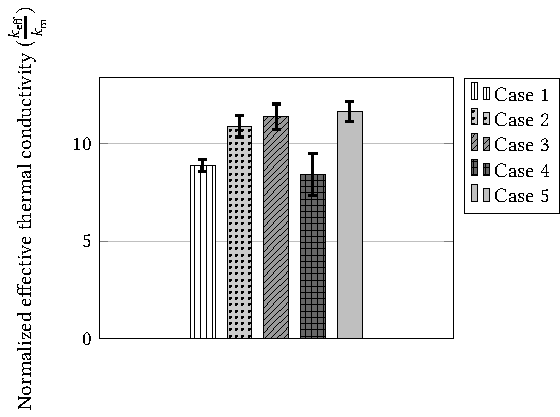
\includegraphics[scale=1]{ddf3_conductivity.pdf}
\caption{Effective conductivity of the composite for four cases of randomly-oriented fibre distributions and an aligned fibre distribution}\label{fig:cond}
\end{figure}%

\red
	Both clustering indices ${\text{[CI]}}_{11}$ and ${\text{[CI]}}_{12}$ had very small values. which indicated that no particular clustering could be detected; all values were of the same order of magnitude. Moreover, the close-to-zero clustering values showed a rather large deviation that is due to the randomness of the data, see Fig.~\ref{fig:CI}. Note that even with such a large variation the clustering indices could not reach any moderate values around 0.4~\autocite{Ranganathan.1990} and do not indicate any clustering. The aligned case showed the lowest clustering value for ${\text{[CI]}}_{11}$ that is attributed to a uniform distribution in terms of number of aligned fibres in every partition.\bl
	
	
%	Comparing the cluster indices does not show a significant difference between all cases except the aligned fibre case, which has the lowest clustering value. This denotes the alignment of the fibres which also results in close-to-zero clustering values with a rather large deviation, see Fig.~\ref{fig:CI}. In addition, all the partitioned cases show higher clustering than randomly distributed fibres without any partitions (case 1). This is another consequence of preventing cross-partition fibre extensions.\bl
	
	\begin{figure}[!h]
	\centering
%	\subfloat[Cluster indexes of the five cases\label{fig:CI}]{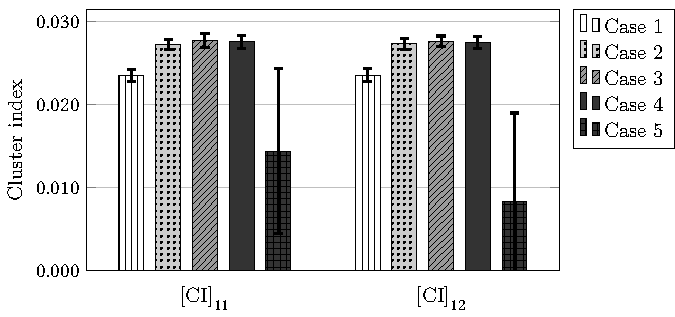
\includegraphics[scale=0.85]{CI}}\\
	\subfloat[Cluster indexes of the five cases\label{fig:CI}]{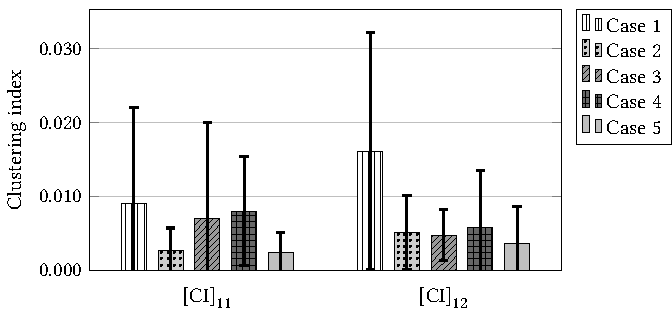
\includegraphics[scale=0.85]{ddf3_cluster}}\\
%	\subfloat[Principal values of the five cases\label{fig:princ}]{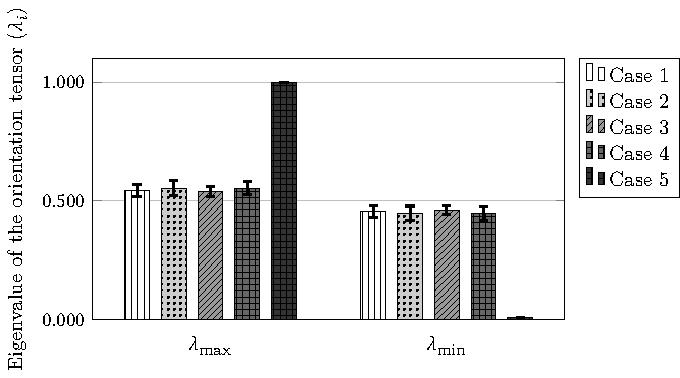
\includegraphics[scale=0.85]{princ}}
	\subfloat[Principal values of the five cases\label{fig:princ}]{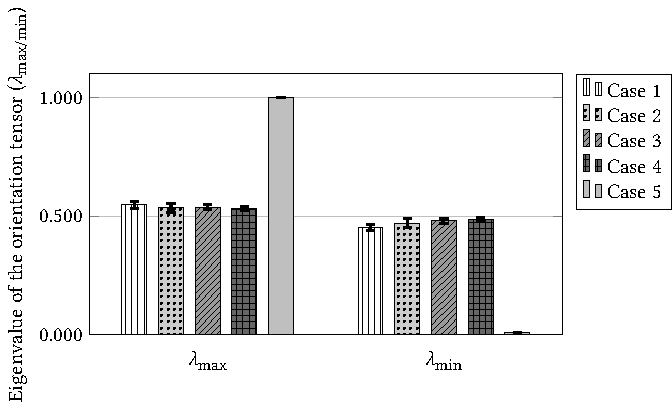
\includegraphics[scale=0.85]{ddf3_lambda}}
	\caption{Summary of the results for parametric analyses}\label{figure:sens}
	\end{figure}%
	
	By carrying out a spectral analysis, the principal directions were obtained, see Table~\ref{table:summary}. Ellipses were used to illustrate the results of principal component analyses. A skewed ellipse denotes a highly oriented state along the maximum principal direction, which in the extreme case becomes a line along the same direction; this is what happened in the case of the aligned fibres, see Fig.~\ref{fig:el_al}. In contrast, the ellipse becomes a circle when there is no preferred orientation state, see Fig.~\ref{fig:el_ra}. In the conducted analyses, since all the random cases were uniformly distributed, values of the same order of magnitude were acquired for the eigenvalues, see Fig.~\ref{fig:princ}. However, the random nature of the distributions can be noted by the obtained diverse principal directions, see Table~\ref{table:summary}.
	
	\begin{figure}[!h]
	\centering
	
	\subfloat[A typical aligned fibre distribution]{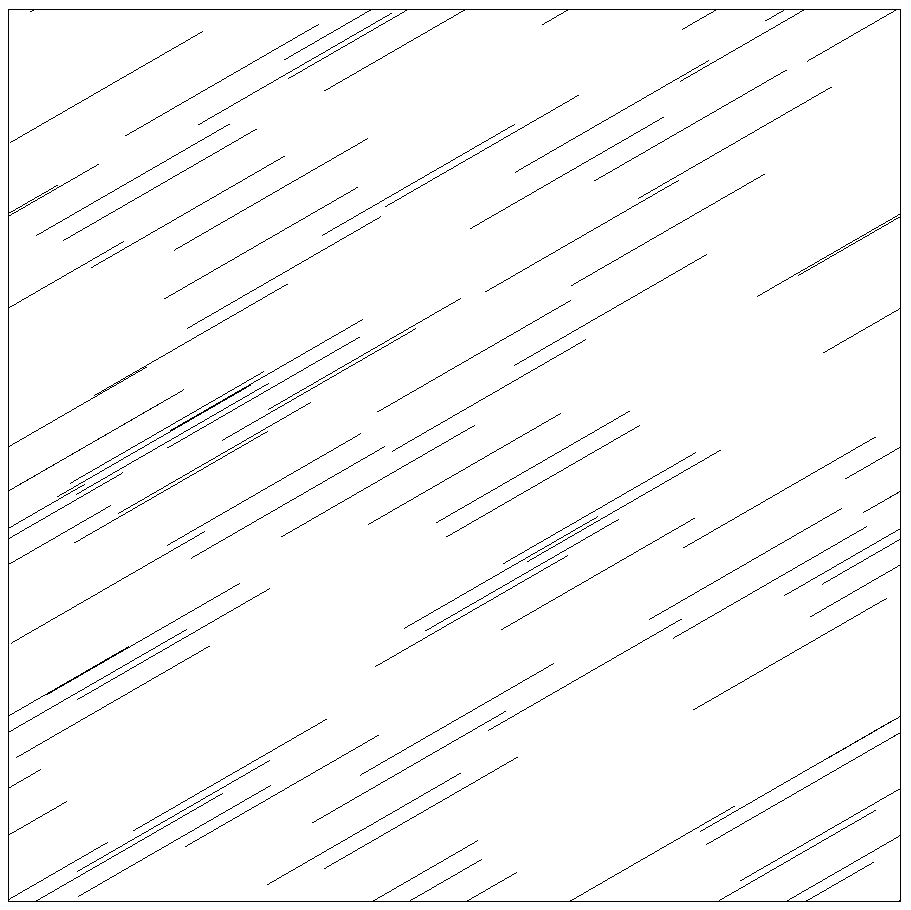
\includegraphics[width=0.22\textwidth]{align}}\hspace{0.15\textwidth}
	\subfloat[Ellipse corresponding to the aligned distribution\label{fig:el_al}]{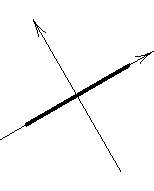
\includegraphics[width=0.22\textwidth]{ddf3_ellipse_aligned.pdf}}\\
	\subfloat[A first case uniform random fibre distribution]{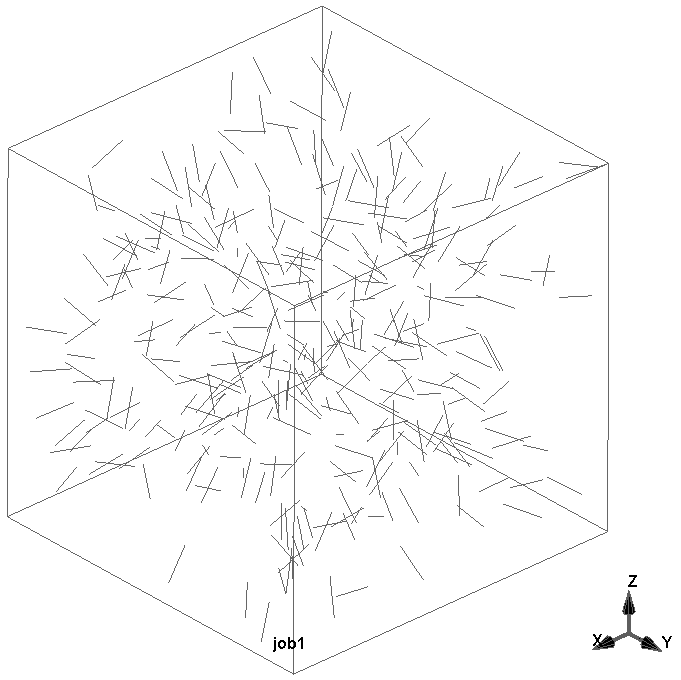
\includegraphics[width=0.22\textwidth]{random}}\hspace{0.15\textwidth}
	\subfloat[Ellipse corresponding to the random distribution\label{fig:el_ra}]{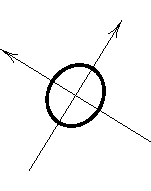
\includegraphics[width=0.22\textwidth]{ddf3_ellipse_random.pdf}}
	\caption{Denoting the principal directions and principal values by ellipses}\label{fig:ellip}
	\end{figure}
	
	\section{Conclusion}
	In conclusion, the finite element method along with the principal component analysis revealed additional information about the anisotropic nature of the randomly-oriented short fibres.\red~In the randomly-oriented cases, the effective thermal conductivity appeared to be largely insensitive to the effects of clustering in the partitions.\bl~However, an extreme aligned case is distinguishable by considering the principal directions and their values. In addition, such eigenvalues can be used to distinguish a uniform fibre distribution from a clustered one. Fibre distribution through partitioning showed a resistance against conductivity in the case of non-uniform distribution of the fibres between partitions along the direction of the thermal gradient. This resulted in more local concentration of the fibres and slightly reduced RVE conductivity. Further investigating the effect of cross-partition penetration is recommended in future studies. Finally, since no direct relation is discovered between the clustering index and the effective conductivity of the RVE, a more local investigation of each case is recommended to consider the effects of the internal anisotropic structure.
	
	\red
	Finally as a corollary, it is worth mentioning that the partitioned RVEs could be used to represent samples of various local phenomena, e.g., fibre clustering or resin-rich regions. Although one RVE is usually used to represent the microstructure, a combination of several RVEs could be a better alternative as it encompasses more of the local variations. The results of the current study showed that altering the parameters of partitioned RVEs could alter the values of effective/apparent properties.
	\bl
	


